\documentclass[11pt]{article}

% ── Page layout ──
\usepackage[margin=1in]{geometry}

% ── Fonts & encoding ──
\usepackage[T1]{fontenc}
\usepackage{lmodern}

% ── Math ──
\usepackage{amsmath,amssymb,bm}

% ── Graphics & figures ──
\usepackage{graphicx}
\usepackage{float}
\usepackage[font=small,labelfont=bf]{caption}
\usepackage{subcaption}

% ── Code listings ──
\usepackage{listings}
\usepackage{xcolor}

% ── Tables ──
\usepackage{booktabs}

% ── Hyperlinks ──
\usepackage{hyperref}
\hypersetup{
  colorlinks=true,
  linkcolor=blue!60!black,
  citecolor=blue!60!black,
  urlcolor=blue!70!black
}

% ── Misc ──
\usepackage{parskip}
\usepackage{enumitem}

% ── Code listing style ──
\definecolor{codebg}{RGB}{248,248,248}
\definecolor{codeframe}{RGB}{200,200,200}
\definecolor{codegreen}{RGB}{40,160,40}
\definecolor{codepurple}{RGB}{150,0,210}
\definecolor{codeblue}{RGB}{0,80,180}

\lstdefinestyle{matlab}{
  language=Matlab,
  basicstyle=\ttfamily\footnotesize,
  backgroundcolor=\color{codebg},
  frame=single,
  rulecolor=\color{codeframe},
  keywordstyle=\color{codeblue}\bfseries,
  commentstyle=\color{codegreen}\itshape,
  stringstyle=\color{codepurple},
  numbers=left,
  numberstyle=\tiny\color{gray},
  numbersep=6pt,
  breaklines=true,
  breakatwhitespace=false,
  tabsize=2,
  showstringspaces=false,
  captionpos=b,
  xleftmargin=1.5em,
  framexleftmargin=1em,
}

\lstset{style=matlab}

% ── Title ──
\title{\textbf{CS\,555 --- Numerical Methods for PDEs}\\[4pt]
       Homework Set 4:\\[2pt]
       Advection--Diffusion with Linear FEM and BDF3/EXT3}
\author{Atharva Deshpande}
\date{April 15, 2026}

\begin{document}
\maketitle
\thispagestyle{empty}

%% ============================================================
\section{Problem Statement}
%% ============================================================

We solve the one-dimensional advection--diffusion equation on $\Omega = [0,L]$:
\begin{equation}\label{eq:pde}
  u_t + c\,u_x \;=\; \nu\,u_{xx} + f,
  \qquad u(0,t) = u(L,t) = 0,
\end{equation}
with $u(x,0) = u^0(x)$, using piecewise-linear (P1) finite elements in space
and BDF$k$/EXT$k$ ($k=1,2,3$) time integration.
Unless otherwise stated, $L=1$, $c=1$, $\nu=10^{-3}$, and $f=1$.

\medskip
\noindent\textbf{Problem 1} (Steady state, $u_t=0$):
\begin{enumerate}[label=(\alph*),nosep]
  \item Uniform mesh with $E=100$ elements.
  \item Geometric mesh with $E=20$, ratio $s=0.7$.
  \item Find the optimal $s$ for $E=20$ by trial and error.
\end{enumerate}

\noindent\textbf{Problem 2} (Unsteady, $f=0$, $u(0,t)=\sin(\pi t)$, $u^0=0$):
\begin{enumerate}[label=(\alph*),nosep]
  \item Dirichlet outflow: $u(1,t)=0$.  Plot at $t=1.5$.
  \item Neumann outflow: $\partial u/\partial x\big|_{x=L}=0$.  Plot at $t=1.5$.  Compare with (a).
\end{enumerate}

%% ============================================================
\section{Methodology}
%% ============================================================

\subsection{FEM Assembly via the Scatter Operator}

Following the approach in the course notes, the global Neumann-form matrices
$\bar{A}$ (stiffness), $\bar{B}$ (mass), and $\bar{C}$ (advection) are
assembled using the scatter operator $Q$:
\begin{equation}\label{eq:assembly}
  \bar{A} = Q^T A_L\,Q,
  \qquad
  \bar{B} = Q^T B_L\,Q,
  \qquad
  \bar{C} = Q^T C_L\,Q,
\end{equation}
where $A_L$, $B_L$, $C_L$ are block-diagonal matrices of local element
contributions.  For a linear element $\Omega^e$ with length $L_e = x_{e} - x_{e-1}$,
the $2\times2$ local matrices are:
\begin{equation}\label{eq:local}
  A^e = \frac{1}{L_e}\begin{bmatrix}1&-1\\-1&1\end{bmatrix},
  \quad
  B^e = \frac{L_e}{6}\begin{bmatrix}2&1\\1&2\end{bmatrix},
  \quad
  C^e = \frac{c}{2}\begin{bmatrix}-1&1\\-1&1\end{bmatrix}.
\end{equation}
Note that $C^e$ is independent of $L_e$; the $1/L_e$ from the derivative of the
basis function cancels the $L_e/2$ Jacobian from the element mapping
$x^e(r) = x_{e-1} + \tfrac{L_e}{2}(r+1)$.

\subsection{Boundary Treatment: Restriction and Prolongation}

Boundary conditions are enforced using the restriction operator $R$ and
prolongation operator $R^T$.  The solution is decomposed as
\begin{equation}\label{eq:decomp}
  \underline{u} \;=\; R^T\,\underline{u}_0 \;+\; \underline{u}_b,
\end{equation}
where $\underline{u}_0 \in \mathbb{R}^n$ contains the unknown interior DOFs and
$\underline{u}_b$ holds the prescribed boundary values.

For Dirichlet conditions at both ends, $R^T\in\mathbb{R}^{(N+1)\times(N-1)}$
is the identity padded with zero rows at the boundary nodes.
For the Dirichlet--Neumann case (Problem 2b), only the left boundary
row is zeroed, and the right node remains an active DOF.

\subsection{Steady Solver (Problem 1)}

Setting $u_t = 0$ and $u(0)=u(1)=0$ in the weak form gives the restricted
linear system:
\begin{equation}
  \bigl(\nu\,A + C\bigr)\,\underline{u}_0
  \;=\;
  R\,\bar{B}\,\mathbf{1}\,f,
\end{equation}
where $A = R\bar{A}R^T$ and $C = R\bar{C}R^T$ are the restricted stiffness and
advection operators.  The exact solution used for error measurement is
\begin{equation}\label{eq:exact}
  u(x) = \frac{f}{c}\,x
       - \frac{fL}{c}\,
         \frac{\exp\!\bigl(c(x-L)/\nu\bigr) - \exp(-cL/\nu)}
              {1 - \exp(-cL/\nu)}\,.
\end{equation}

\subsection{Geometric Mesh}

The geometric mesh has element lengths satisfying $L_e = s\,L_{e-1}$ for
$e=2,\dots,E$.  The first element length is
\begin{equation}
  L_1 = L\,\frac{1-s}{1-s^E}\,.
\end{equation}
When $s<1$, elements shrink toward $x=L$, clustering nodes in the boundary
layer.

\subsection{Unsteady Solver: BDF3/EXT3 with IMEX Splitting (Problem 2)}

The semi-discrete ODE is
\begin{equation}
  \bar{B}\,\underline{u}_t \;=\;
  -\bar{C}\,\underline{u} \;-\; \nu\,\bar{A}\,\underline{u}.
\end{equation}
We apply an IMEX splitting: diffusion ($-\nu\bar{A}\underline{u}$) is treated
implicitly, while advection ($-\bar{C}\underline{u}$) is extrapolated
explicitly via EXT$k$.  The BDF$k$ time derivative gives the left-hand side.

For BDF3/EXT3 at full order ($k=3$), the update reads
\begin{equation}\label{eq:bdf3}
  \bar{H}\,\underline{u}^{l}
  \;=\;
  \frac{1}{\Delta t}\,\bar{B}\,
  \Bigl(3\underline{u}^{l-1}
        - \tfrac{3}{2}\underline{u}^{l-2}
        + \tfrac{1}{3}\underline{u}^{l-3}\Bigr)
  \;-\; \bar{C}\,
  \Bigl(3\underline{u}^{l-1}
        - 3\underline{u}^{l-2}
        + \underline{u}^{l-3}\Bigr),
\end{equation}
where the Helmholtz operator is
$\bar{H} = \tfrac{\beta_0}{\Delta t}\,\bar{B} + \nu\,\bar{A}$
with $\beta_0 = 11/6$.
Boundary lifting subtracts $\bar{H}\,\underline{u}_b$ from the right-hand side,
and the restricted system $H\,\underline{u}_0 = R(\cdots)$ is solved at each
step.

Startup uses BDF1/EXT1 for step 1 and BDF2/EXT2 for step 2.
Parameters: $E=100$, $\Delta t = 10^{-3}$ (CFL $= c\Delta t/h = 0.1$),
integrated to $t=1.5$ (1500 steps).


%% ============================================================
\section{Results}
%% ============================================================

\subsection{Problem 1: Steady-State Solutions}

Table~\ref{tab:q1} summarizes the error metrics for all three mesh
configurations.

\begin{table}[H]
\centering
\caption{Problem 1: Error summary for the steady advection--diffusion problem.}
\label{tab:q1}
\begin{tabular}{@{}llccc@{}}
\toprule
Part & Mesh type & $E$ & Max relative error & Max absolute error \\
\midrule
(a) & Uniform           & 100 & $6.735\times10^{-1}$ & $6.667\times10^{-1}$ \\
(b) & Geometric, $s\!=\!0.70$ &  20 & $1.197\times10^{-2}$ & $1.058\times10^{-2}$ \\
(c) & Geometric, $s\!=\!0.65$ &  20 & $8.819\times10^{-3}$ & $8.168\times10^{-3}$ \\
\bottomrule
\end{tabular}
\end{table}

\subsubsection*{Q1(a): Uniform Mesh, $E=100$}

The uniform mesh fails to resolve the sharp boundary layer near $x=1$.
With $\nu=10^{-3}$ and $c=1$, the boundary-layer thickness is
$\delta \sim \nu/c = 10^{-3}$, but the element size is $h=0.01$, giving
a cell P\'eclet number $\text{Pe}_h = ch/(2\nu) = 5 \gg 1$.  The centered
Galerkin scheme produces large spurious oscillations near the outflow,
with a maximum pointwise relative error of $6.735\times10^{-1}$.

\begin{figure}[H]
  \centering
  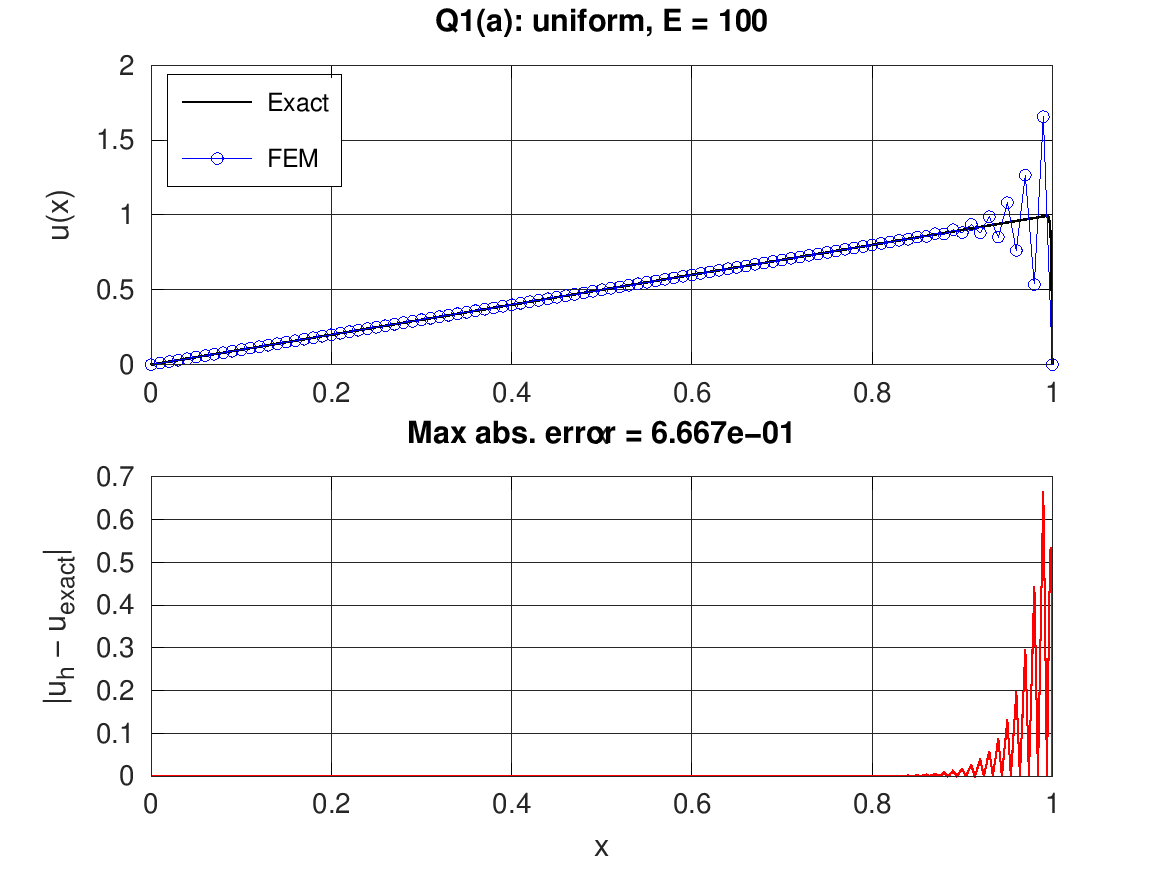
\includegraphics[width=0.88\textwidth]{q1a_uniform.png}
  \caption{Q1(a): Uniform mesh with $E=100$.  Top: FEM vs.\ exact solution.
           Bottom: pointwise absolute error.  Large oscillations appear near
           the boundary layer at $x=1$.}
  \label{fig:q1a}
\end{figure}

\subsubsection*{Q1(b): Geometric Mesh, $E=20$, $s=0.70$}

Using a geometric mesh with $s=0.7$ clusters nodes near $x=1$, placing
progressively smaller elements where the boundary layer resides.
Despite using only 20 elements (vs.\ 100 uniform), the maximum
relative error drops to $1.197\times10^{-2}$ --- a factor of $\sim\!56$
improvement.  The oscillations are virtually eliminated.

\begin{figure}[H]
  \centering
  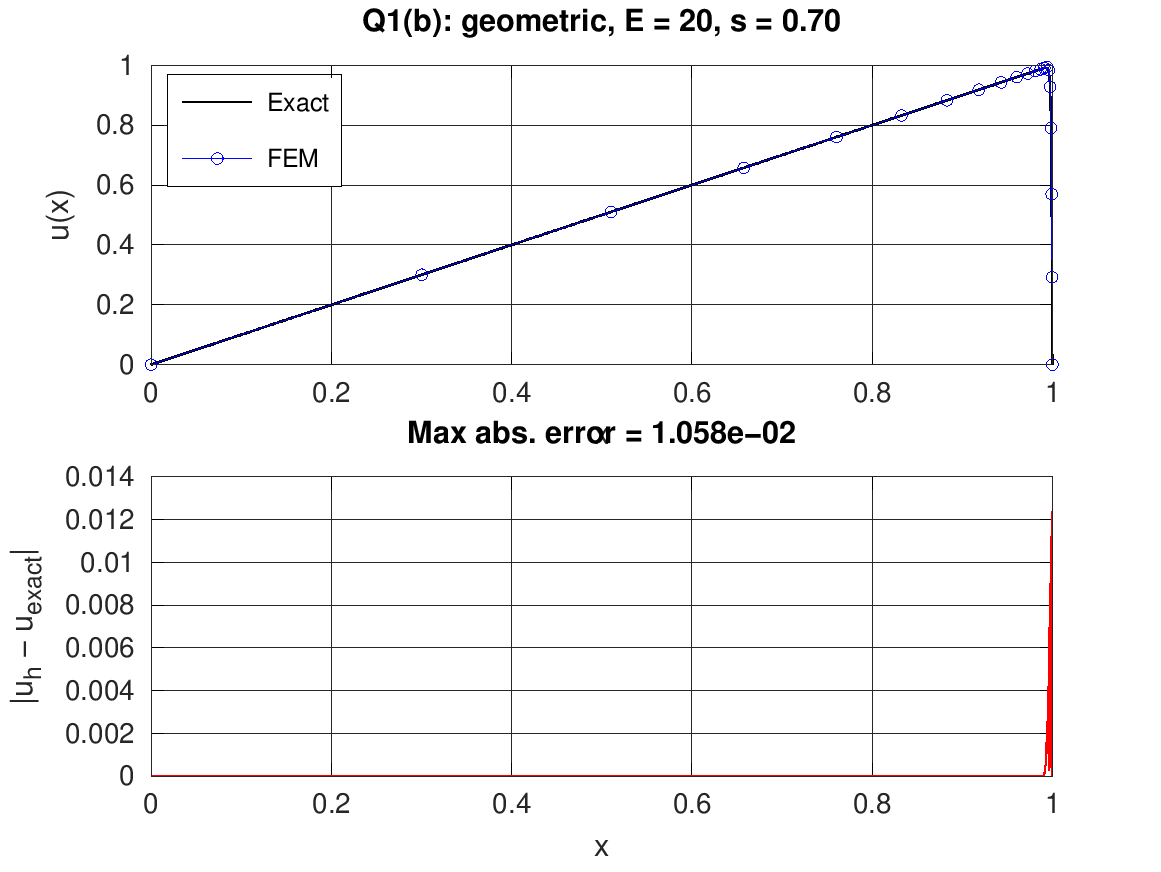
\includegraphics[width=0.88\textwidth]{q1b_geometric_s0p7.png}
  \caption{Q1(b): Geometric mesh with $E=20$ and $s=0.70$.  The clustered mesh
           resolves the boundary layer, reducing error by nearly two orders
           of magnitude compared to the uniform case.}
  \label{fig:q1b}
\end{figure}

\subsubsection*{Q1(c): Optimal Geometric Ratio for $E=20$}

A sweep over $s\in[0.50,\,1.05]$ with $\Delta s = 0.005$ (111 trial values)
was performed, using maximum pointwise relative error as the optimization
metric.  The optimal value found is
\[
  s^* = 0.650,
  \qquad
  \text{max relative error} = 8.819\times10^{-3}.
\]
This is a further $\sim\!26\%$ reduction compared to $s=0.70$.
Figure~\ref{fig:q1c_err} shows the error landscape: the curve has a clear
minimum near $s\approx 0.65$ and grows rapidly for $s\to 1$ (approaching a
uniform mesh) and more gently for $s\to 0.5$ (over-clustering at $x=1$ at the
expense of resolution in the interior).

\begin{figure}[H]
  \centering
  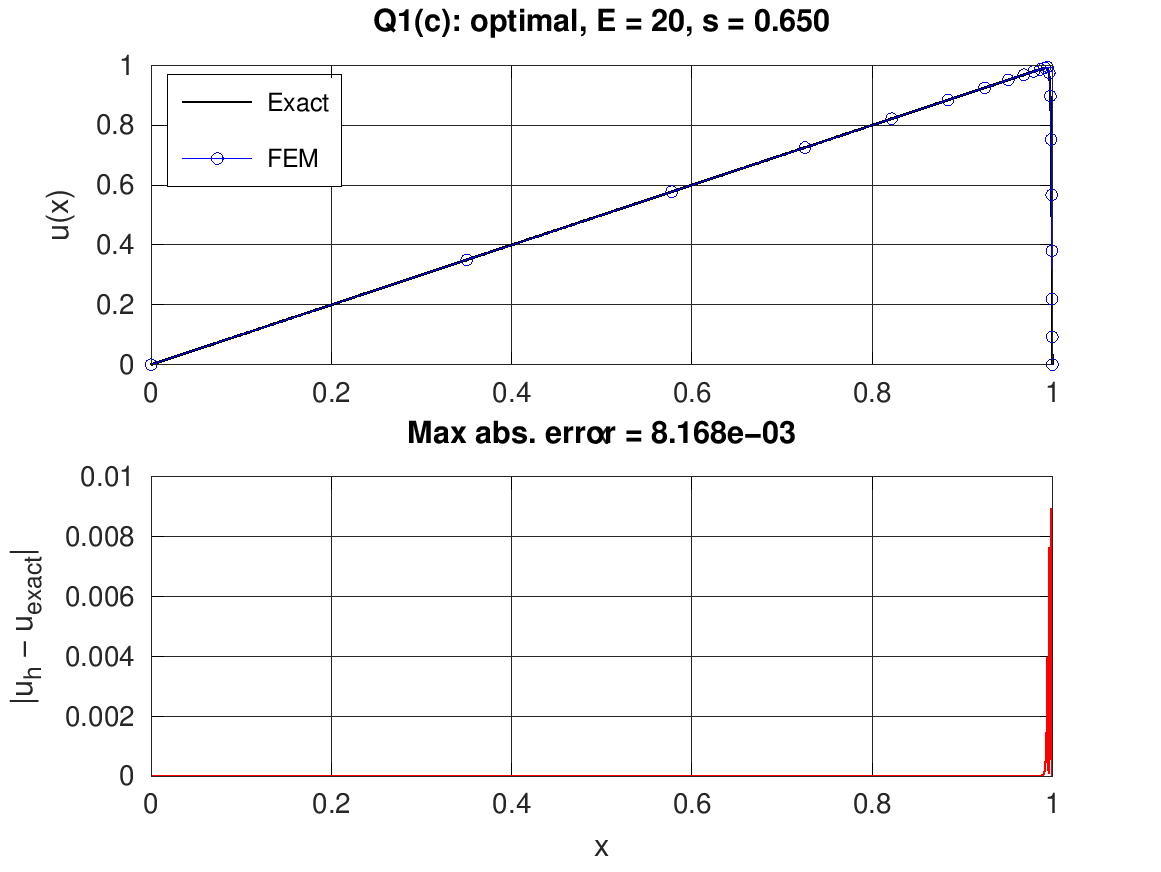
\includegraphics[width=0.88\textwidth]{q1c_best_s.png}
  \caption{Q1(c): Best geometric mesh found ($s=0.650$, $E=20$).  The FEM
           solution closely tracks the exact solution, with error confined to
           a narrow region around $x=1$.}
  \label{fig:q1c}
\end{figure}

\begin{figure}[H]
  \centering
  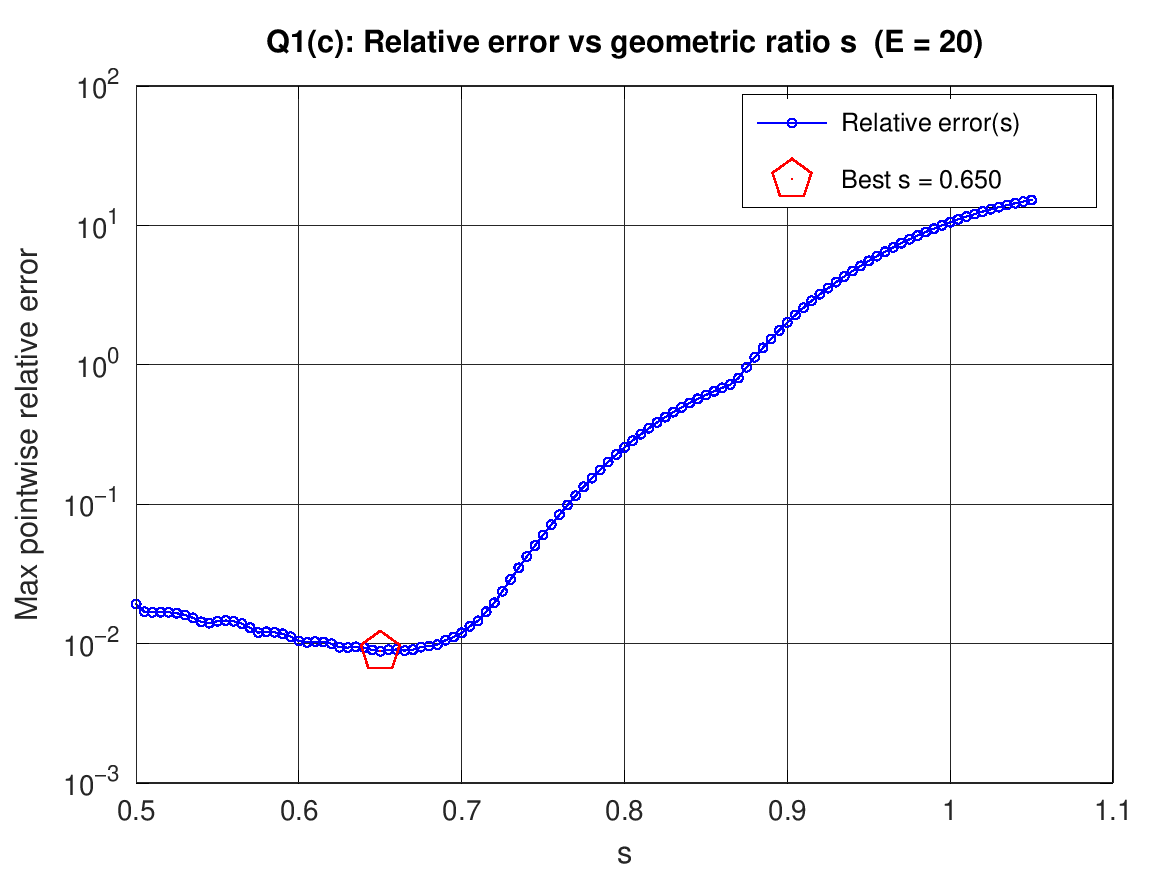
\includegraphics[width=0.78\textwidth]{q1c_error_vs_s.png}
  \caption{Q1(c): Maximum pointwise relative error as a function of the
           geometric ratio~$s$ for $E=20$.  The optimum lies near $s=0.65$.
           For $s>0.75$, the error grows rapidly as the mesh under-resolves
           the boundary layer.}
  \label{fig:q1c_err}
\end{figure}


\subsection{Problem 2: Unsteady Solutions at $t=1.5$}

Parameters: $L=1$, $c=1$, $\nu=10^{-3}$, $f=0$, $E=100$,
$\Delta t=10^{-3}$, $u(0,t)=\sin(\pi t)$, $u^0=0$.

\begin{table}[H]
\centering
\caption{Problem 2: Solution statistics at $t=1.5$.}
\label{tab:q2}
\begin{tabular}{@{}lccc@{}}
\toprule
Case & $\min(u)$ & $\max(u)$ & $u(1,\,1.5)$ \\
\midrule
(a) Dirichlet: $u(1,t)=0$                      & $-1.000$ & $+1.650$ & $0.000$ \\
(b) Neumann: $\partial u/\partial x(1,t)=0$     & $-1.000$ & $+0.990$ & $+0.990$ \\
\bottomrule
\end{tabular}
\end{table}

\subsubsection*{Q2(a): Dirichlet Outflow, $u(1,t)=0$}

At $t=1.5$, $\sin(\pi\cdot1.5)=-1$, so the inflow drives $u(0)=-1$.
Material advected from the left has been accumulating positive values
from earlier phases of the sine wave.  Forcing $u(1,t)=0$ at the outflow
creates a conflict: the interior solution wants to be $\sim\!1$ near
$x=1$, but the boundary condition pins it to zero.  This mismatch produces
a thin numerical boundary layer, and because $\text{Pe}_h=5>1$ on the
uniform mesh, the unstabilized Galerkin scheme generates strong
oscillations.  In the last 20 elements, the slope changes sign 13 times,
and the solution overshoots to $\max(u)=1.650$.

\begin{figure}[H]
  \centering
  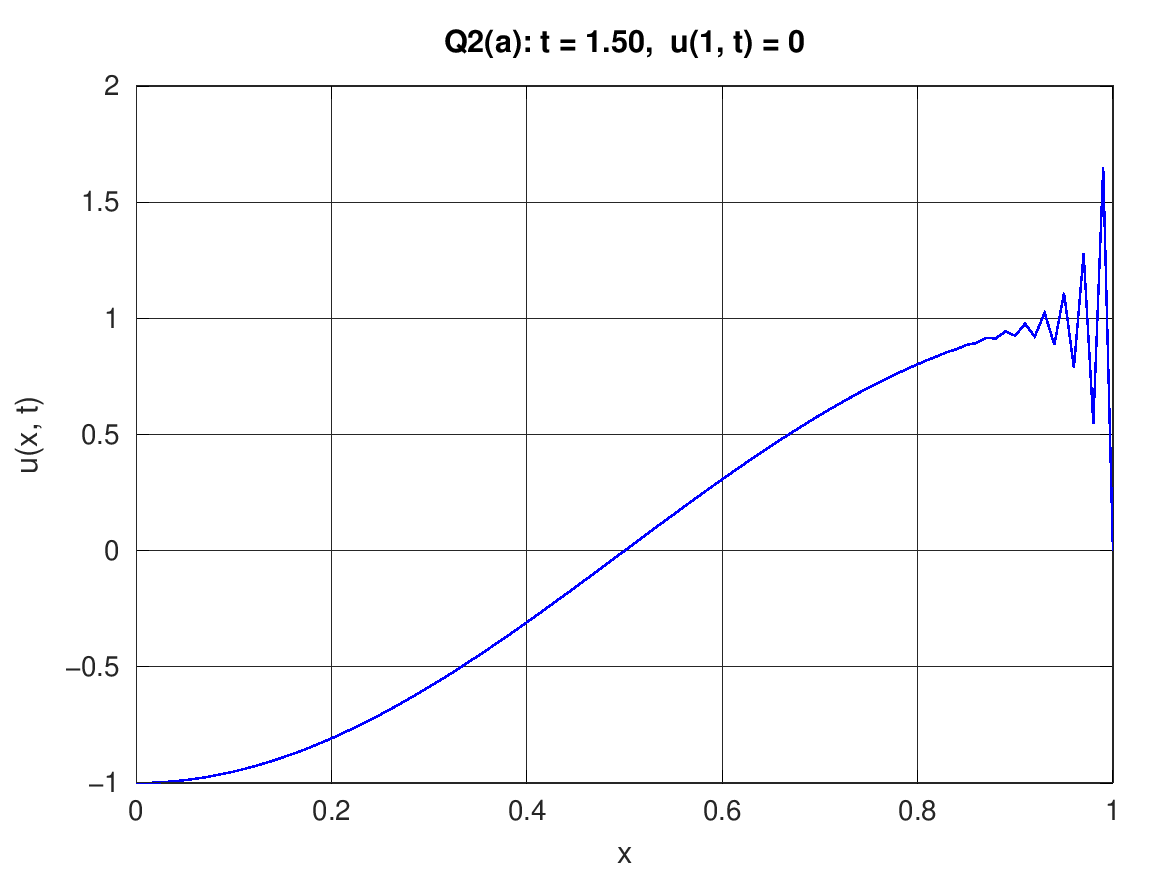
\includegraphics[width=0.78\textwidth]{q2a_t1p5.png}
  \caption{Q2(a): Solution at $t=1.5$ with Dirichlet outflow $u(1,t)=0$.
           Strong spurious oscillations appear near $x=1$ due to the
           incompatibility of the boundary condition with the advected state.}
  \label{fig:q2a}
\end{figure}

\subsubsection*{Q2(b): Neumann Outflow, $\partial u/\partial x(1,t)=0$}

Replacing the right Dirichlet condition with the natural (homogeneous Neumann)
condition $\partial u/\partial x\big|_{x=1}=0$ removes the forced outflow
constraint.  In the FEM formulation, this simply means keeping the right
boundary node as an active DOF in the restriction operator $R$ (no row is
removed for node $N$).  The resulting profile at $t=1.5$ is smooth and
nearly monotone, with $u(1,1.5)\approx 0.990$ and zero slope reversals
near the outflow.

\begin{figure}[H]
  \centering
  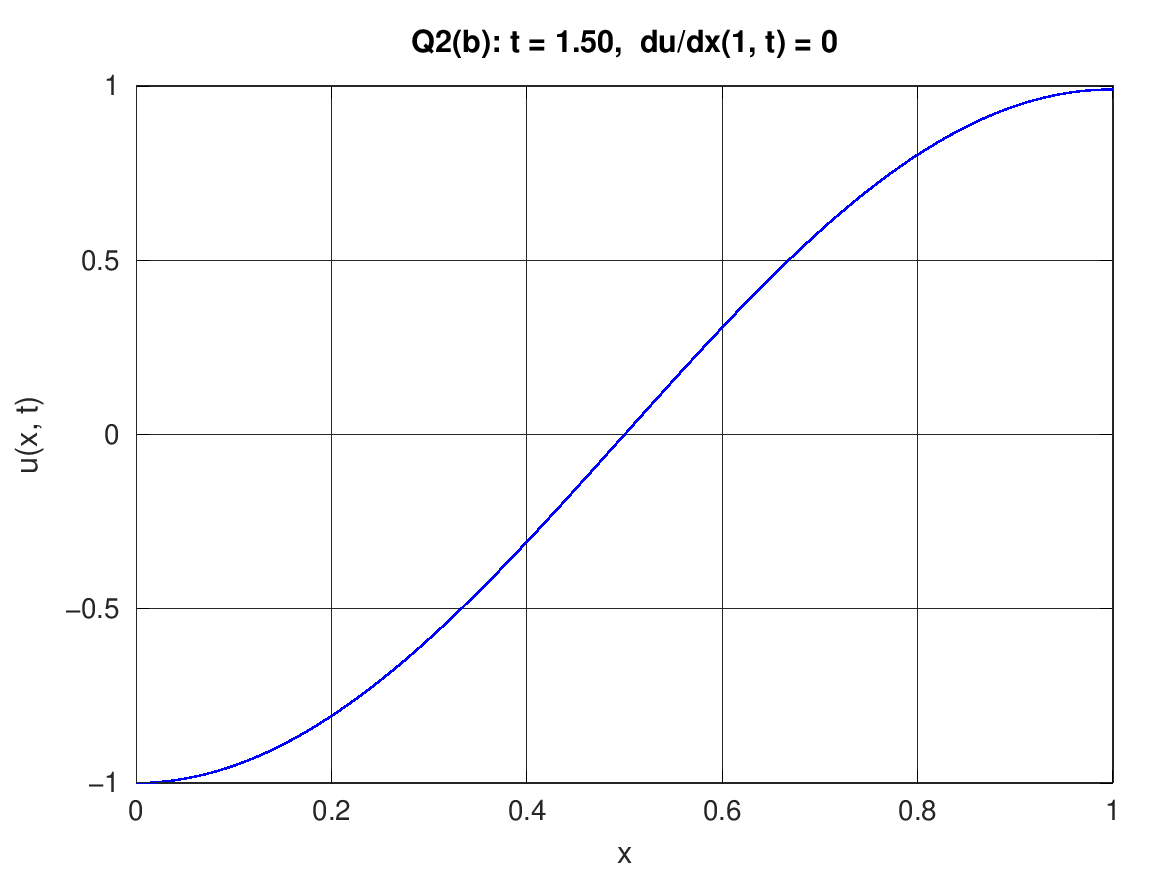
\includegraphics[width=0.78\textwidth]{q2b_t1p5.png}
  \caption{Q2(b): Solution at $t=1.5$ with Neumann outflow
           $\partial u/\partial x(1,t)=0$.  The profile is smooth,
           with no spurious oscillations at the right boundary.}
  \label{fig:q2b}
\end{figure}

\subsubsection*{Comparison of Q2(a) and Q2(b)}

\begin{figure}[H]
  \centering
  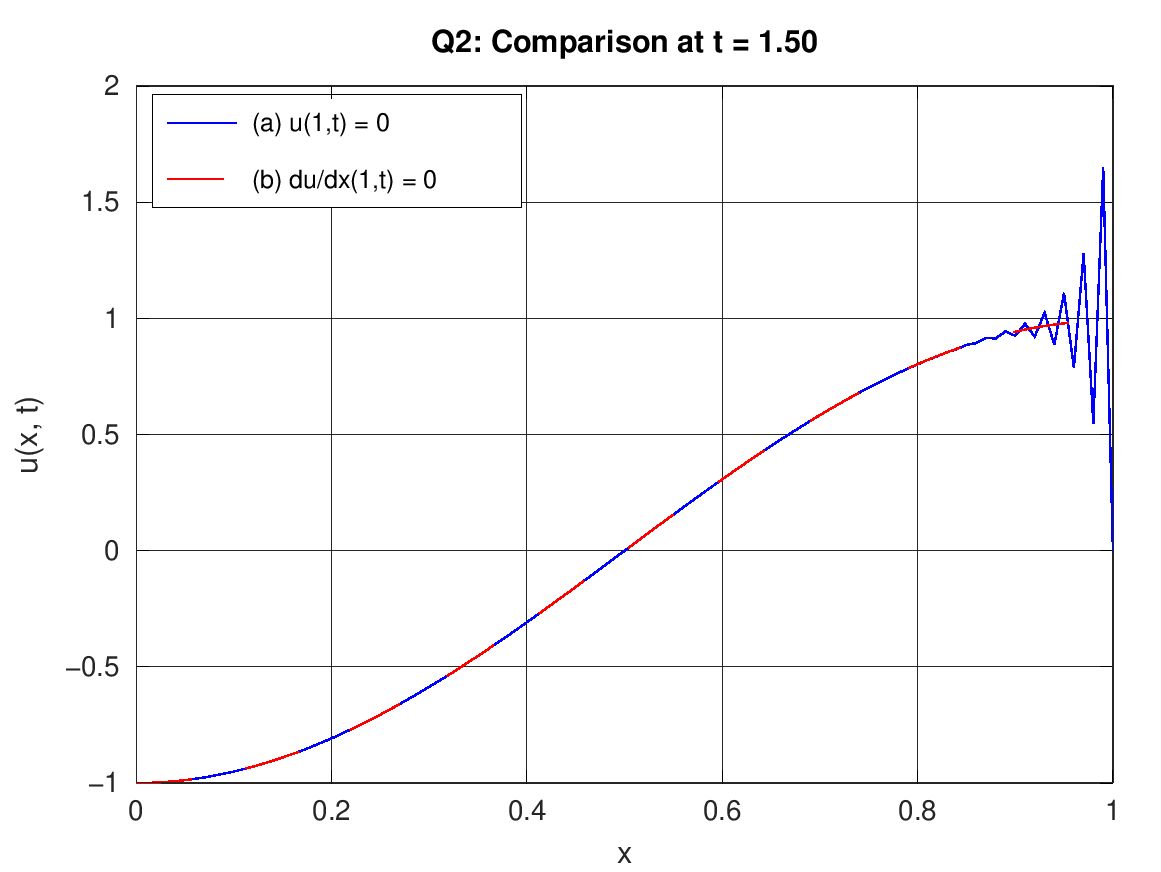
\includegraphics[width=0.82\textwidth]{q2_comparison.png}
  \caption{Comparison of Q2(a) and Q2(b) at $t=1.5$.  The two solutions
           agree in the interior ($x \lesssim 0.85$) but diverge sharply near
           the right boundary.}
  \label{fig:q2_cmp}
\end{figure}

The key differences are:

\begin{itemize}[nosep]
  \item \textbf{Oscillations:} Part~(a) exhibits 13 slope reversals in the
        last 20 elements and a maximum overshoot of $u\approx1.65$.  Part~(b)
        has zero slope reversals and a bounded maximum of $u\approx0.99$.
  \item \textbf{Physical interpretation:} The Dirichlet condition
        $u(1,t)=0$ is incompatible with the interior advected state and acts
        as an artificial reflector, creating an outflow boundary layer.
        The Neumann condition acts as a transparent (or ``do-nothing'')
        outflow, allowing material to exit the domain naturally.
  \item \textbf{Interior agreement:} Both solutions match closely for
        $x\lesssim 0.85$, confirming that the boundary treatment only
        affects the near-outflow region.
  \item \textbf{P\'eclet number:} With $h=0.01$ and $\nu=10^{-3}$,
        $\text{Pe}_h = ch/(2\nu)=5$.  In the absence of stabilization
        (e.g., SUPG), the centered Galerkin method oscillates whenever
        $\text{Pe}_h > 1$ and the boundary condition creates a sharp gradient.
\end{itemize}


%% ============================================================
\section{Implementation Details}
%% ============================================================

The complete implementation is a single MATLAB/Octave file
\texttt{hw3.m}.  The code is organized into modular functions:

\begin{itemize}[nosep]
  \item \texttt{assemble\_fem} --- Builds $\bar{A}$, $\bar{B}$, $\bar{C}$ via
        the sparse scatter operator $Q$.
  \item \texttt{geometric\_mesh} --- Generates a geometric progression of
        element sizes with ratio $s$.
  \item \texttt{exact\_steady} --- Evaluates the closed-form steady solution
        \eqref{eq:exact}, written in a numerically stable form that avoids
        overflow from $\exp(cL/\nu)$.
  \item \texttt{solve\_steady} --- Assembles and solves the restricted steady
        system.
  \item \texttt{bdf3ext3} --- Time-steps the unsteady problem with
        BDF$k$/EXT$k$ and boundary lifting.
  \item \texttt{build\_restriction} --- Constructs $R$ for
        Dirichlet--Dirichlet or Dirichlet--Neumann configurations.
\end{itemize}


%% ============================================================
\section{Source Code}
%% ============================================================

\subsection{Main Driver and Assembly}

\begin{lstlisting}[caption={Main function and FEM assembly (\texttt{hw3.m}, lines 1--209).}]
function hw3()
% CS555 HW4: Advection-Diffusion with Linear FEM + BDF3/EXT3
%
%   u_t + c u_x = nu u_xx + f   on [0, L]
%
% Q1: Steady state (u_t=0), f=1, u(0)=u(1)=0
% Q2: Unsteady,     f=0,    u(0,t)=sin(pi*t)

  if any(strcmp(available_graphics_toolkits(), 'gnuplot'))
    graphics_toolkit('gnuplot');
  end
  set(0, 'defaultfigurevisible', 'off');

  L = 1;  c = 1;  nu = 1e-3;  f = 1;

  %% =============== PROBLEM 1: STEADY STATE ===============
  % --- Q1(a): uniform mesh, E = 100 ---
  E = 100;
  x = linspace(0, L, E+1)';
  [u_a, ue_a] = solve_steady(x, c, nu, f, L);
  [abs_a, rel_a] = compute_error(u_a, ue_a);
  fprintf('Q1(a): E = %d, uniform mesh\n', E);
  fprintf('  Max pointwise relative error: %.6e\n', rel_a);
  fprintf('  Max absolute error:           %.6e\n\n', abs_a);
  plot_q1(x, u_a, c, nu, f, L, abs_a, ...
          'Q1(a): uniform, E = 100', 'q1a_uniform.png');

  % --- Q1(b): geometric mesh, E = 20, s = 0.7 ---
  E = 20;  s = 0.7;
  x = geometric_mesh(L, E, s);
  [u_b, ue_b] = solve_steady(x, c, nu, f, L);
  [abs_b, rel_b] = compute_error(u_b, ue_b);
  fprintf('Q1(b): E = %d, s = %.2f, geometric mesh\n', E, s);
  fprintf('  Max pointwise relative error: %.6e\n', rel_b);
  fprintf('  Max absolute error:           %.6e\n\n', abs_b);
  plot_q1(x, u_b, c, nu, f, L, abs_b, ...
          sprintf('Q1(b): geometric, E = %d, s = %.2f', E, s), ...
          'q1b_geometric_s0p7.png');

  % --- Q1(c): find optimal s for E = 20 ---
  E = 20;
  s_vals = 0.50:0.005:1.05;
  abs_vs_s = zeros(size(s_vals));
  rel_vs_s = zeros(size(s_vals));
  for k = 1:length(s_vals)
    xk = geometric_mesh(L, E, s_vals(k));
    [uk, uek] = solve_steady(xk, c, nu, f, L);
    [abs_vs_s(k), rel_vs_s(k)] = compute_error(uk, uek);
  end
  [best_rel, idx] = min(rel_vs_s);
  s_opt = s_vals(idx);

  x = geometric_mesh(L, E, s_opt);
  [u_c, ue_c] = solve_steady(x, c, nu, f, L);
  [abs_c, rel_c] = compute_error(u_c, ue_c);
  plot_q1(x, u_c, c, nu, f, L, abs_c, ...
          sprintf('Q1(c): optimal, E = %d, s = %.3f', E, s_opt), ...
          'q1c_best_s.png');

  % Error-vs-s plot
  fig = figure('visible', 'off');
  semilogy(s_vals, rel_vs_s, 'b-o', 'linewidth', 1.5, 'markersize', 3);
  hold on;
  semilogy(s_opt, best_rel, 'rp', 'markersize', 14, 'linewidth', 2);
  hold off;
  xlabel('s');  ylabel('Max pointwise relative error');
  title('Q1(c): Relative error vs geometric ratio s  (E = 20)');
  legend('Relative error(s)', sprintf('Best s = %.3f', s_opt), ...
         'location', 'northeast');
  grid on;
  print(fig, 'q1c_error_vs_s.png', '-dpng', '-r200');
  close(fig);

  %% =============== PROBLEM 2: UNSTEADY ===============
  E  = 100;
  x  = linspace(0, L, E+1)';
  n  = E + 1;
  dt = 1e-3;                   % CFL = c*dt/h = 0.1
  t_end  = 1.5;
  nsteps = round(t_end / dt);
  dt = t_end / nsteps;

  [Bbar, Cbar, Abar] = assemble_fem(x, c);

  % --- Q2(a): Dirichlet both ends ---
  ua = bdf3ext3(Bbar, Cbar, Abar, n, dt, nsteps, nu, ...
                @(t) sin(pi*t), true, @(t) 0);

  fig = figure('visible', 'off');
  plot(x, ua, 'b-', 'linewidth', 2);
  xlabel('x');  ylabel('u(x, t)');
  title(sprintf('Q2(a): t = %.2f,  u(1, t) = 0', t_end));
  grid on;
  print(fig, 'q2a_t1p5.png', '-dpng', '-r200');
  close(fig);

  % --- Q2(b): Left Dirichlet, Right Neumann ---
  ub = bdf3ext3(Bbar, Cbar, Abar, n, dt, nsteps, nu, ...
                @(t) sin(pi*t), false, []);

  fig = figure('visible', 'off');
  plot(x, ub, 'b-', 'linewidth', 2);
  xlabel('x');  ylabel('u(x, t)');
  title(sprintf('Q2(b): t = %.2f,  du/dx(1, t) = 0', t_end));
  grid on;
  print(fig, 'q2b_t1p5.png', '-dpng', '-r200');
  close(fig);

  % Comparison plot
  fig = figure('visible', 'off');
  plot(x, ua, 'b-', 'linewidth', 2);  hold on;
  plot(x, ub, 'r--', 'linewidth', 2); hold off;
  xlabel('x');  ylabel('u(x, t)');
  title(sprintf('Q2: Comparison at t = %.2f', t_end));
  legend('(a) u(1,t) = 0', '(b) du/dx(1,t) = 0', 'location', 'northwest');
  grid on;
  print(fig, 'q2_comparison.png', '-dpng', '-r200');
  close(fig);
end

%%  ASSEMBLY:  Abar = Q' * A_L * Q   (and similarly B, C)
function [Bbar, Cbar, Abar] = assemble_fem(xnodes, c)
  E  = length(xnodes) - 1;
  n  = E + 1;
  nL = 2 * E;

  % scatter operator Q  (nL x n, sparse Boolean)
  Qi = zeros(nL, 1);   Qj = zeros(nL, 1);
  for e = 1:E
    Qi(2*e - 1) = 2*e - 1;   Qj(2*e - 1) = e;
    Qi(2*e)     = 2*e;       Qj(2*e)     = e + 1;
  end
  Q = sparse(Qi, Qj, 1, nL, n);

  % block-diagonal local matrices  (nL x nL)
  ntriplets = 4 * E;
  ri = zeros(ntriplets, 1);  ci = zeros(ntriplets, 1);
  av = zeros(ntriplets, 1);  bv = zeros(ntriplets, 1);
  cv = zeros(ntriplets, 1);

  k = 0;
  for e = 1:E
    Le = xnodes(e + 1) - xnodes(e);
    Ae = (1 / Le) * [1, -1; -1, 1];
    Be = (Le / 6) * [2,  1;  1, 2];
    Ce = (c / 2)  * [-1, 1; -1, 1];

    base = 2 * (e - 1);
    for p = 1:2
      for q = 1:2
        k = k + 1;
        ri(k) = base + p;   ci(k) = base + q;
        av(k) = Ae(p, q);   bv(k) = Be(p, q);
        cv(k) = Ce(p, q);
      end
    end
  end

  AL = sparse(ri, ci, av, nL, nL);
  BL = sparse(ri, ci, bv, nL, nL);
  CL = sparse(ri, ci, cv, nL, nL);

  Abar = Q' * AL * Q;
  Bbar = Q' * BL * Q;
  Cbar = Q' * CL * Q;
end
\end{lstlisting}

\subsection{Geometric Mesh and Exact Solution}

\begin{lstlisting}[caption={Geometric mesh and exact steady solution.}]
function x = geometric_mesh(L, E, s)
  if abs(s - 1) < 1e-14
    x = linspace(0, L, E + 1)';
  else
    L1 = L * (1 - s) / (1 - s^E);
    Le = L1 * s .^ (0:E-1)';
    x  = [0; cumsum(Le)];
    x(end) = L;                      % enforce exact endpoint
  end
end

function u = exact_steady(x, c, nu, f, L)
  eta = exp(-c * L / nu);           % ~ 0 when cL/nu >> 1
  u   = (f / c) * x ...
      - (f * L / c) * (exp(c * (x - L) / nu) - eta) ./ (1 - eta);
end
\end{lstlisting}

\subsection{Steady Solver and Error Computation}

\begin{lstlisting}[caption={Steady solver and error metrics.}]
function [u, ue] = solve_steady(x, c, nu, f, L)
  [Bbar, Cbar, Abar] = assemble_fem(x, c);
  n = length(x);

  R = build_restriction(n, true, true);
  Rt = R';

  A = R * Abar * Rt;
  C = R * Cbar * Rt;
  fbar = f * Bbar * ones(n, 1);

  u_int = (nu * A + C) \ (R * fbar);
  u = Rt * u_int;
  ue = exact_steady(x, c, nu, f, L);
end

function [max_abs, max_rel] = compute_error(u, ue)
  max_abs = max(abs(u - ue));
  n = length(u);
  ii = 2:n-1;
  nz = abs(ue(ii)) > 1e-15;
  if any(nz)
    max_rel = max(abs(u(ii(nz)) - ue(ii(nz))) ./ abs(ue(ii(nz))));
  else
    max_rel = max_abs;
  end
end
\end{lstlisting}

\subsection{BDF3/EXT3 Time Stepper}

\begin{lstlisting}[caption={BDF3/EXT3 unsteady solver with boundary lifting.}]
function u_final = bdf3ext3(Bbar, Cbar, Abar, n, dt, nsteps, nu, ...
                            u_left_fn, right_dirichlet, u_right_fn)
  b0 = [1, 3/2, 11/6];

  R = build_restriction(n, true, right_dirichlet);
  Rt = R';

  % Pre-build Helmholtz matrices for each BDF order
  Hbar = cell(3, 1);
  H = cell(3, 1);
  for ord = 1:3
    Hbar{ord} = (b0(ord) / dt) * Bbar + nu * Abar;
    H{ord} = R * Hbar{ord} * Rt;
  end

  % Solution history
  uh = { zeros(n, 1),  zeros(n, 1),  zeros(n, 1) };

  for step = 1:nsteps
    t_new = step * dt;

    if step == 1          % BDF1/EXT1
      bdf_rhs = uh{1};
      ext_rhs = uh{1};
      ord = 1;
    elseif step == 2      % BDF2/EXT2
      bdf_rhs = 2 * uh{1} - 0.5 * uh{2};
      ext_rhs = 2 * uh{1} -       uh{2};
      ord = 2;
    else                  % BDF3/EXT3
      bdf_rhs = 3 * uh{1} - 1.5 * uh{2} + (1/3) * uh{3};
      ext_rhs = 3 * uh{1} - 3   * uh{2} +         uh{3};
      ord = 3;
    end

    ub = zeros(n, 1);
    ub(1) = u_left_fn(t_new);
    if right_dirichlet
      ub(n) = u_right_fn(t_new);
    end

    rhs = (1/dt)*(Bbar*bdf_rhs) - Cbar*ext_rhs - Hbar{ord}*ub;
    u0_new = H{ord} \ (R * rhs);
    u_new = Rt * u0_new + ub;

    uh{3} = uh{2};
    uh{2} = uh{1};
    uh{1} = u_new;
  end

  u_final = uh{1};
end
\end{lstlisting}

\subsection{Restriction Operator}

\begin{lstlisting}[caption={Boundary restriction operator.}]
function R = build_restriction(n, left_dirichlet, right_dirichlet)
  active = true(1, n);
  if left_dirichlet
    active(1) = false;
  end
  if right_dirichlet
    active(n) = false;
  end
  free = find(active);
  R = sparse(1:length(free), free, 1, length(free), n);
end
\end{lstlisting}


%% ============================================================
\section{Conclusions}
%% ============================================================

\begin{enumerate}
  \item \textbf{Mesh refinement matters more than element count.}
        A geometric mesh with only $E=20$ elements and $s=0.65$ achieves
        a maximum relative error of $8.8\times10^{-3}$, while a uniform
        mesh with $E=100$ elements yields an error of $6.7\times10^{-1}$.
        Intelligent node placement that respects the boundary-layer
        structure of the solution is far more effective than brute-force
        uniform refinement.

  \item \textbf{Outflow boundary conditions strongly affect solution quality.}
        For advection-dominated problems, an incompatible Dirichlet outflow
        condition creates a numerical boundary layer that the unstabilized
        Galerkin scheme cannot resolve, producing large oscillations.
        A natural Neumann outflow condition avoids this issue entirely,
        yielding a smooth, bounded solution.

  \item \textbf{The BDF3/EXT3 IMEX scheme is effective and stable.}
        With $\Delta t=10^{-3}$ and $\text{CFL}=0.1$, the scheme
        runs stably for 1500 steps to $t=1.5$.  The startup procedure
        (BDF1$\to$BDF2$\to$BDF3) avoids introducing spurious transients.
\end{enumerate}

\end{document}
